\section*{Aufgabe 3}
\subsection*{a)}
In der Abbildung \ref{fig:euler} ist das exakte Ergebnis und der numerische Weg mit dem (symmetrischen)
Euler-Verfahren dargestellt.
Das Zeitintervall $t \in [0, 10]$ wurde bei beiden Verfahren extra in nur 150 Schritte unterteilt,
damit die Abweichungen klar zu sehen sind.
Bei dem Euler-Verfahren sind kaum Abweichungen zu erkennen, wobei 
bei dem symmetrischen Euler-Verfahren vor allen Dingen bei großen Werten von $t$ 
starke Oszillationen zu verzeichen sind.
\begin{figure}
    \centering
    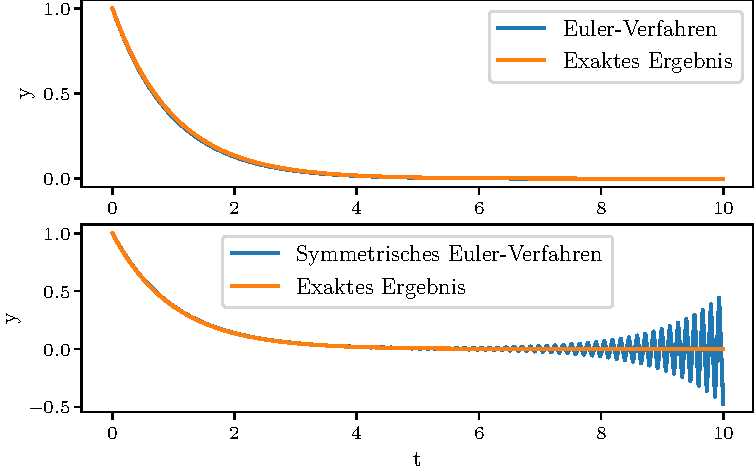
\includegraphics[width = 0.95 \textwidth]{build/ex_3_plot_symm.pdf}
    \caption{Exakte und mit dem (symmetrischen) Euler-Verfahren (150 Schritte) ermittelte
    Ergebnisse.}
    \label{fig:euler}
\end{figure}